\documentclass[ebook,12pt,oneside,openany]{memoir}

% For putting figure 'H'(ere)
\usepackage{float}

% Listings
\usepackage{listings}

% \includegraphics
\usepackage{ifluatex}
\ifluatex
  \usepackage{pdftexcmds}
  \makeatletter
  \let\pdfstrcmp\pdf@strcmp
  \let\pdffilemoddate\pdf@filemoddate
  \makeatother
\fi

\usepackage{hyperref}

\usepackage{amsmath}

% TikZ
\usepackage{tikz}
\usepackage{tkz-graph}
\usepackage{pgf}
\usetikzlibrary{arrows,automata}

% Style of code
% From http://r.789695.n4.nabble.com/How-to-nicely-display-R-code-with-the-LaTeX-package-listings-tp4648110.html
\usepackage{fancyvrb} 
\definecolor{codegreen}{rgb}{0,0.6,0}
\definecolor{codegray}{rgb}{0.5,0.5,0.5}
\definecolor{codepurple}{rgb}{0.58,0,0.82}
\definecolor{backcolor}{rgb}{0.95,0.95,0.92}
\lstdefinestyle{mystyle}{
  language=R,% set programming language
  basicstyle=\ttfamily\small,% basic font style
  commentstyle=\color{gray},% comment style
  numbers=left,% display line numbers on the left side
  numberstyle=\scriptsize,% use small line numbers
  numbersep=10pt,% space between line numbers and code
  tabsize=2,% sizes of tabs
  showstringspaces=false,% do not replace spaces in strings by a certain character
  captionpos=b,% positioning of the caption below
  breaklines=true,% automatic line breaking
  escapeinside={(*}{*)},% escaping to LaTeX
  fancyvrb=true,% verbatim code is typset by listings
  extendedchars=false,% prohibit extended chars (chars of codes 128--255)
  literate={"}{{\texttt{"}}}1{<-}{{$\bm\leftarrow$}}1{<<-}{{$\bm\twoheadleftarrow$}}1
  {~}{{$\bm\sim$}}1{<=}{{$\bm\le$}}1{>=}{{$\bm\ge$}}1{!=}{{$\bm\neq$}}1{^}{{$^{\bm\wedge}$}}1,% item to replace, text, length of chars
  alsoletter={.<-},% becomes a letter
  alsoother={$},% becomes other
  otherkeywords={!=, ~, $, \&, \%/\%, \%*\%, \%\%, <-, <<-, /},% other keywords
  deletekeywords={c}% remove keywords 
}
\lstset{style=mystyle}

\title{Travis TeX to EPUB example 1}

\author{Rich\`el J.C. Bilderbeek} 
\begin{document}

\maketitle

\tableofcontents

\begin{abstract}

This is a \LaTeX document showing code, as used in \href{https://github.com/richelbilderbeek/travis_tex_to_epub_example_1}{travis\_tex\_to\_epub\_example\_1}.

\end{abstract}

\section{Introduction}

This document compares a PDF and EPUB version of the same TeX file.
The results differ. The reason is given \href{https://ebooks.stackexchange.com/questions/6632/calibre-viewer-displays-books-wrong}{here}
and boils down to that Calibre extracts text from images/tables/etc. as much as it can.
If you really want an image, supply a PNG.

The PDF version does show an abstract. 
The EPUB version does not show an abstract.

The PDF version does show a Table of Content. 
The EPUB version does not do so implicity: one can select the section from a sidebar.

The PDF version allows a proper citation of beastier\cite{beastier}.
The EPUB version does not show the citation, displayed as '\verb;[1];' after the word 'beastier' in the previous sentence.

The PDF version does show a bibliography. 
The EPUB version does not show a bibliography.

\section{Plain code}

\begin{lstlisting}
#include <iostream>

int main()
{
  std::cout << "Hello world\n";
}
\end{lstlisting}

The PDF version show the code above in monospace, with its first line greyed out, and with numbered lines.
The EPUB shows the code in monospace.

\section{Added a frame and specific markup}

% language=C++: highlight code fitting to the C++ programming language
% showstringspaces=false: keep a blank space between 'Hello' and 'world'
% frame=single: put a box around the code
\begin{lstlisting}[language=C++,showstringspaces=false,frame=single,label=lst:code_with_frame]
#include <iostream>

int main()
{
  std::cout << "Hello world\n";
}
\end{lstlisting}

The PDF version of the code above shows a frame around the code, code is monospace, first line is black, lines are numbered.
The EPUB version shows the code in monospace, without a frame.

The PDF version allows to refer to figure \ref{lst:code_with_frame} and places a number there.
The EPUB version show the LaTeX code to refer to the listing in verbatim.

\section{Listing with caption}

% language=C++: highlight code fitting to the C++ programming language
% showstringspaces=false: keep a blank space between 'Hello' and 'world'
% frame=single: put a box around the code
\begin{lstlisting}[
  label=lst:caption,
  caption=Label of code with added label and caption,
  captionpos=below,
  language=C++,showstringspaces=false,frame=single
]
#include <iostream>

int main()
{
  std::cout << "Hello world\n";
}
\end{lstlisting}

The PDF version shows the caption underneath the listing laid out differently than the main text.
The EPUB version shows the caption as any default text.

\section{An equation}

\begin{equation}
  \Delta r=\frac{ln\left(\frac{L(T)}{L(\frac{1}{2}T)}\right)-ln\left(\frac{L(\frac{1}{2}T)}{L(0)}\right)}{ln\left(\frac{L(T)}{L(\frac{1}{2}T)}\right)+ln\left(\frac{L(\frac{1}{2}T)}{L(0)}\right)}
  \label{eq:delta_r}
\end{equation}

The PDF version shows the equation rendered well.
The EPUB version show the LaTeX code to write the equation verbatim. 

\section{A PNG figure}

Without a \verb;figure; environment:

\includegraphics[scale=1.0]{TravisCI.png}

The PDF version and EPUB version display the figure identically.

With a \verb;figure; environment:
	
\begin{figure}[H]
  \centering
  \includegraphics[scale=1.0]{TravisCI.png}
  \caption{Label of figure in a figure environment}
  \label{fig:png}
\end{figure}

The PDF version centers the image and its label.
The EPUB version puts the image at the left of the text, shows the caption with the default font.

\section{An SVG figure}

Cannot do this with additional help, as the SVG needs to be converted to EPS first.

\section{A TikZ figure}

%%%%%%%%%%%%%%%%%%%%%%%%%%%%%%%%%%%%%%%%%%%%%%%%%%%%%%%%%%%%%%%%%%%%%%%%%%%%%%%%
\begin{figure}[H]
  \centering
  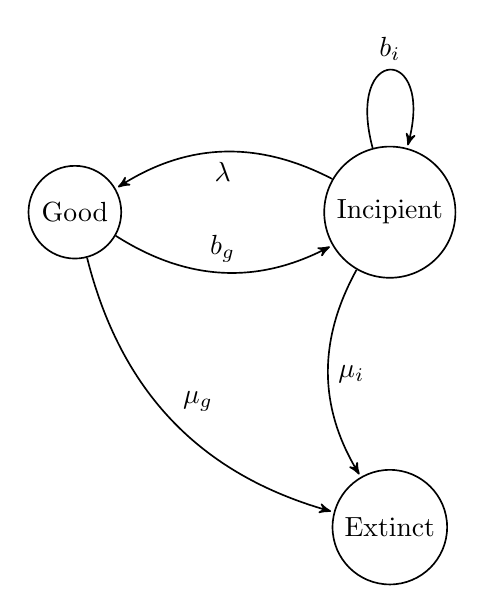
\begin{tikzpicture}[->,>=stealth',shorten >=1pt,auto,node distance=4cm, semithick]   
  \tikzstyle{every state}=[]
  \node[state] (A)              {Good};   
  \node[state] (B) [right of=A] {Incipient};   
  \node[state] (C) [below of=B] {Extinct};   
  \path (A) edge [bend right] node {$b_g$} (B)
        (A) edge [bend right] node {$\mu_g$} (C)
        (B) edge [loop above] node {$b_i$} (B)
        (B) edge [bend right] node {$\lambda$} (A)
        (B) edge [bend right] node {$\mu_i$} (C); 
  \end{tikzpicture}
  \caption{Label of the TikZ figure}
  \label{fig:tikz}
\end{figure}
%%%%%%%%%%%%%%%%%%%%%%%%%%%%%%%%%%%%%%%%%%%%%%%%%%%%%%%%%%%%%%%%%%%%%%%%%%%%%%%%

The PDF version renders the TikZ image well.
The EPUB version shows the TikZ code verbatim.

\section{A table}

\begin{table}[H]
  \begin{tabular}{ | l || c | r | }
    \hline                       
    1 & 2 & 3 \\
    \hline                       
    \hline                       
    4 & 5 & 6 \\
    7 & 8 & 9 \\
    \hline  
  \end{tabular}
  \label{tbl:my_table}
  \caption{The caption of the table}
\end{table}

The PDF version shows the table with both horizontal and vertical lines. The caption is displayed below the table.
The EPUB shows the table without horizontal nor vertical lines. The first row shows text in bold face. The label is displayed verbatim below the table. The caption is showed above the table.

\bibliographystyle{plain}
\bibliography{example}

\end{document}